\documentclass[tikz,border=2pt]{standalone}
\usepackage{amsmath,amssymb}
\usetikzlibrary{arrows.meta,positioning,calc}
\definecolor{ink}{HTML}{0B0B0B}
\definecolor{ink2}{HTML}{52514E}
\definecolor{blue}{HTML}{2A78D6}
\definecolor{orange}{HTML}{EB6834}
\definecolor{grey}{HTML}{8A8984}
\begin{document}
\hyphenpenalty=10000
\exhyphenpenalty=10000
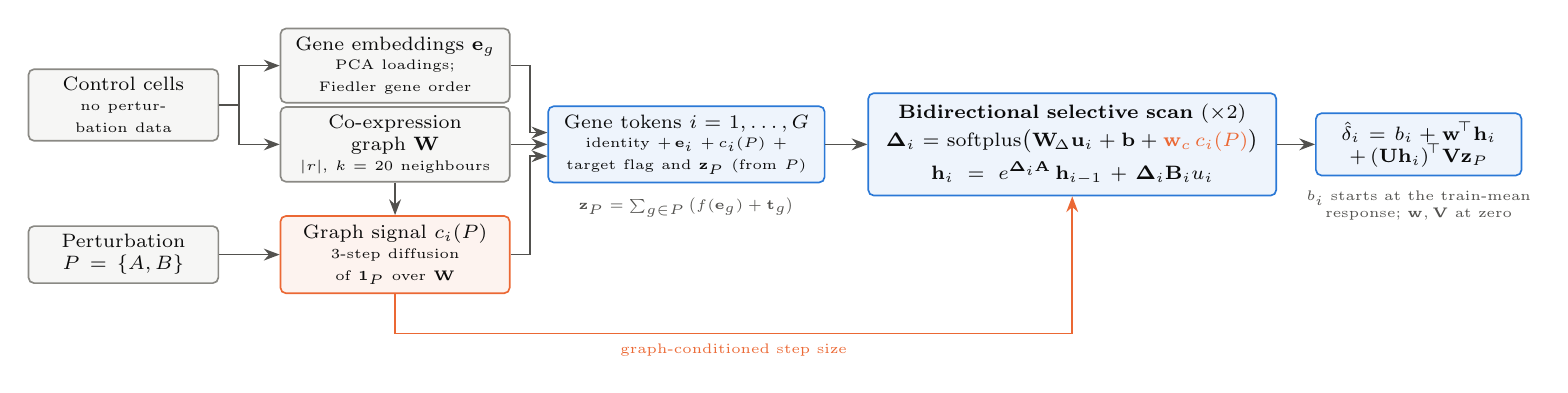
\begin{tikzpicture}[
  font=\scriptsize, >=Stealth, line width=0.6pt,
  box/.style={draw=#1, rounded corners=2pt, align=center, inner sep=3pt, fill=#1!8, text=ink},
  lbl/.style={text=ink2, font=\tiny, align=center},
  arr/.style={->, draw=ink2}]

% column 1: raw inputs
\node[box=grey, text width=22mm] (ctrl) at (0, 0.55) {Control cells\\[-1pt]{\tiny no perturbation data}};
\node[box=grey, text width=22mm] (pert) at (0,-1.35) {Perturbation\\$P=\{A,B\}$};

% column 2: derived inputs (all from control cells, identical across splits)
\node[box=grey, text width=27mm] (emb) at (3.45, 1.05) {Gene embeddings $\mathbf{e}_g$\\[-1pt]{\tiny PCA loadings; Fiedler gene order}};
\node[box=grey, text width=27mm] (W)   at (3.45, 0.05) {Co-expression graph $\mathbf{W}$\\[-1pt]{\tiny $|r|$, $k=20$ neighbours}};
\node[box=orange, text width=27mm] (c) at (3.45,-1.35) {Graph signal $c_i(P)$\\[-1pt]{\tiny 3-step diffusion of $\mathbf{1}_P$ over $\mathbf{W}$}};
\draw[arr] (ctrl.east) -- ++(2.5mm,0) |- (emb.west);
\draw[arr] (ctrl.east) -- ++(2.5mm,0) |- (W.west);
\draw[arr] (pert.east) -- (c.west);
\draw[arr] (W.south) -- (c.north);

% column 3: tokens
\node[box=blue, text width=33mm] (tok) at (7.15, 0.05)
  {Gene tokens $i=1,\dots,G$\\[-1pt]{\tiny identity $+\,\mathbf{e}_i$ $+\,c_i(P)$ $+$ target flag and $\mathbf{z}_P$ (from $P$)}};
\node[lbl, below=0.6mm of tok] {$\mathbf{z}_P=\sum_{g\in P}\big(f(\mathbf{e}_g)+\mathbf{t}_g\big)$};
\draw[arr] (emb.east) -- ++(2.5mm,0) |- ([yshift=1.5mm]tok.west);
\draw[arr] (W.east) -- (tok.west);
\draw[arr] (c.east) -- ++(2.5mm,0) |- ([yshift=-1.5mm]tok.west);

% column 4: graph-conditioned SSM
\node[box=blue, text width=49mm, inner sep=4pt] (ssm) at (12.05, 0.05)
  {\textbf{Bidirectional selective scan} ($\times 2$)\\[2pt]
   $\boldsymbol{\Delta}_i=\mathrm{softplus}\big(\mathbf{W}_{\!\Delta}\mathbf{u}_i+\mathbf{b}+\textcolor{orange}{\mathbf{w}_c\,c_i(P)}\big)$\\[2pt]
   $\mathbf{h}_i=e^{\boldsymbol{\Delta}_i\mathbf{A}}\,\mathbf{h}_{i-1}+\boldsymbol{\Delta}_i\mathbf{B}_i u_i$};
\draw[arr] (tok.east) -- (ssm.west);
\draw[->, draw=orange] (c.south) -- ++(0,-5mm) -| (ssm.south) node[pos=0.25, below, font=\tiny, text=orange] {graph-conditioned step size};

% column 5: readout
\node[box=blue, text width=24mm] (out) at (16.45, 0.05)
  {$\hat\delta_i=b_i+\mathbf{w}^{\!\top}\mathbf{h}_i$\\$+\,(\mathbf{U}\mathbf{h}_i)^{\!\top}\mathbf{V}\mathbf{z}_P$};
\draw[arr] (ssm.east) -- (out.west);
\node[lbl, below=0.6mm of out] {$b_i$ starts at the train-mean\\response; $\mathbf{w},\mathbf{V}$ at zero};
\end{tikzpicture}
\end{document}
